\documentclass[oneside,letterpaper]{memoir}

\usepackage[utf8]{inputenc}

\setlength{\parindent}{0pt}
\usepackage{listings}
\usepackage{geometry}               		
\geometry{letterpaper}                   	
\usepackage{graphicx}				
\usepackage{amssymb}
\usepackage{amsmath}
\usepackage{commath}
\usepackage{physics}
\usepackage[utf8]{inputenc}
\usepackage{amsthm}
\usepackage[english]{babel}

\usepackage{blkarray}

\usepackage{float}

\newtheorem{proposition}{Proposition}
\newtheorem{theorem}{Theorem}
\newtheorem{corollary}{Corollary}[theorem]
\newtheorem{lemma}[theorem]{Lemma}

\theoremstyle{definition}
\newtheorem{definition}{Definition}
\newtheorem{remark}{Remark}
\newtheorem{example}{Example}

\DeclareMathOperator{\ran}{\text{ran }} %% Needed in Aug12_2016
\DeclareMathOperator{\im}{\text{im }}
\DeclareMathOperator{\lrarrow}{\leftrightarrow}


\title{CPSC 589 - Assignment 2}
\date{Winter 2018}
\author{Scott Saunders - 10163541}

\begin{document}
\maketitle
\begin{enumerate}
\item
(10 marks) For the case of a planar B-spline curve, does symmetry of the control polygon with respect to the y-axis imply the same symmetry for the curve? \\

No. \\
%For the base case, for two points to be symmetric you have two points:(x,y),(-x,y)  (from defn. of symmetric), and  will be at the 0-axis \\
%For incrementing the number of points, any odd number of points would have the middle-point on the y-axsis.
%By induction, over the degree of the B-spline curve,
%While, for more points, and higher-degree curves, the 

Assuming uniform knot sequences, this is.
$P_0 = (-1,-1), P_1 = (0,0) , P_2 = (1,-1)$, is symmetric, as is \\
//$P_0 = (-1,1), P_1 = (1,1), P_2 = (-1,1), P_3 = (1,1)$  \\

However, with a different knot sequence: {0,0,1}
This is no longer symmetric.

\newpage

\item
(20 marks) A closed mesh (i.e. no boundary vertices) is saved in a half-edge data structure. For a given face f , write, in pseudocode, an algorithm that

\begin{enumerate}
\item finds all faces adjacent to f \\
\begin{verbatim}
let f be our current face,
e = f.edge;
adj<faces>;
do
  adj.push_back( e.pair.face );
  e=e.next;
while(e != f.getEdge);

return adj;
\end{verbatim}
This simply iterates of each edge of the face, and appends it's face to the returned value.\\
\item all vertices that are on f or connected to f by an edge. \\
\begin{verbatim}
let f be our current face,
e = f.edge;
verts<vertices>;

do
  verts.push_back(e.source);
  e2 = e;
  do
    verts.push_back(e2.source);
    e2 = e2.next.pair
  while ( e2 != e || e2 != e.next.pair)
  e=e.next;
while(e != f.getEdge);

return verts;
\end{verbatim}
Outer loop, iterates over all all vertices that are on f, and adds them. \\
Inner loop, iterates over all edges of a given vertex, and adds their vertices (except the one we're currently one, and it's next one, as that'll get added in the next iteration of the outer loop)
\end{enumerate}

\newpage

\item
a)% no ideas.
% You can tell how smooth based on hwen eigen values start to repeat. (two or more)
% so for quadratic 1/2 1/4 1/4 (only two spots, then rest are same)
% so for cubic 1 1/2 1/4 1/8  1/8 (three spots?
% so 1 1/2 1/6... so not as smooth
You can tell how smooth it is based on when the eigen values start repeating: \\
Where quadratic is $1/2, 1/4, 1/4$ \\
and cubic is $1, 1/2, 1/4, 1/8, 1/8$ \\
Hence, this provided filiter is less-smooth than cubic, and smoother than quadratic. \\
b)
Yes, all weights of the filter are sum-to-one in a row \\

\newpage

\item
(15 marks) Consider a mesh with e edges, v vertices, and f faces. Compute the new number
of edges (e 0 ), vertices (v 0 ), and faces (f 0 ) after one level of subdivision in the cases of the
Loop and Doo-Sabin methods. Show your calculations. Assume the mesh doesn’t have any
boundaries.
\begin{itemize}
\item Doo-Sabin method: \\
From the origonal paper: \\
"In this process, 3 types of new faces can be formed: \\
a) Type F: A 5-sided face will give a new smaller 5-sided face within itself and bears a smiliar shape, this type of new face is termed Type F (fromed by face). \\
b) Type V: A vecterx common to 4 faces, i.e. a corner where 3 faces joined togeather having three common boundaries, will produce a 3-sided face, this is Termed type V, (fromed by vertex). \\
c) Type E: On each common boundary of two adjacent faces, a 4-sided face will be formed, this is termed Type E (fromed by edge). \\

  The new polyhedron will consist of these 3 types of new faces. A n-sided face will provide a basis for a smaller n-sided F type new face, it will remain n-sided as the subdivision carries on and will gradually converge to the centroid and diminish to an acceptable size. A common edge will always produce a 4-sided new face, and m-spoked vertex will produce a m-sided V type face, which will, in turn, become the basis of a smaller m-sided F type face in the next subdivision process." \\

Taking this togeather, you have: \\
$f' = f + e + v$ \\

(Again from the paper, as I have read it and cannot un-read it) \\
Each e will give a 4-sided polygon with 4 new verticies, however any two adjacent edges on a face will generate only one new vertex on that face, therefore the number of new verticies formed will be: \\
$v' = 4 e / 2 = 2e$ \\
Note: This can also be verified by the expansion/shrinking method of thinking about it: As each edge is shrunk/extended, each end of each old-edge, now creates a vertex, independed of any other edge. This gives $v' = 2e$. \\

Finnally, we use Euler's formula for polyhedron: $F+V-E=2$ to get the number of edges: \\
$e'=f'+v'-2$ \\
$e'=f+e+v + 2e + -2$ \\
$e'= f + v + 3e -2$ \\


In summary: \\
$f' = f + e + v$ \\
$v' = 2e$ \\
$e'= f + v + 3e -2$ \\

\item Loop method: \\
%Each edge is divided in half, giving  \\
%$e' = 2e + (e/3)*3 = 2e+ e = 3e;$ \\
Each edge is dubled, and each face procudes 3 new edges giving:
$f' = 2e + 3*f$ \\
Each vertex is kept, while each edge is cut in half with a new vertex giving:
$v' = v+e;$ \\
Each face procudes 3 new ones, and persists through giving:
 $f' = f*4$ \\
%so using euler's formula to verify on a single triangle: \\
%$F+V-E=2$ \\
%Single triangle: e=3; f=1, v=3;\\
%1+3-3=2
\end{itemize}

\newpage

\item
(10 marks) The first quadratic B-spline basis function defining on positive integer numbers (knot sequence) is given as: \\
\begin{enumerate}
\item Show that N_{0,3} (u) is really a third order spline function (verify the necessary properties only at u = 0). \\

At $N_{0,3}$, we must show that it is continious, and hence a spline function: \\
At $u=0$:
$C^0 : 0 = u^2/2 \to  0  = 0$
$C^1 : 0 = u^2/2 \to  0  = 0$
$C^2 : 0 = u \to 0 = 0$
$C^3 : 0 = 0 \to 0 = 0$

Hence, it has $c^3$ continuity at $u=0$, which is all that was requested. \\

\item Determine $N_{5,3} (u)$ (try to use $N+{0,3} (u)$). Show your work. \\
As the above equation is for the uniform-knot sequence, and there isn't any reason to assume it is not uniform, we can $N_{i,3}(u) = N_{0,3}(u-i)$. Which gives us: \\
$N_{5,3}(u) = N_{0,3}(u - 5)$ \\
\end{enumerate}

\newpage

\item
(20 marks) For Catmull-Clark subdivision, we would like to subdivide only a particular area
of the mesh using an adaptive subdivision method.
\begin{enumerate}
\item Extend the simple (naive) T-junction insertion method of Adaptive Loop subdivision to create an Adaptive Catmull-Clark subdivision. Draw a figure to support your description. \\
Note: the picture is taken from the CPSC589 notes, page 126. \\
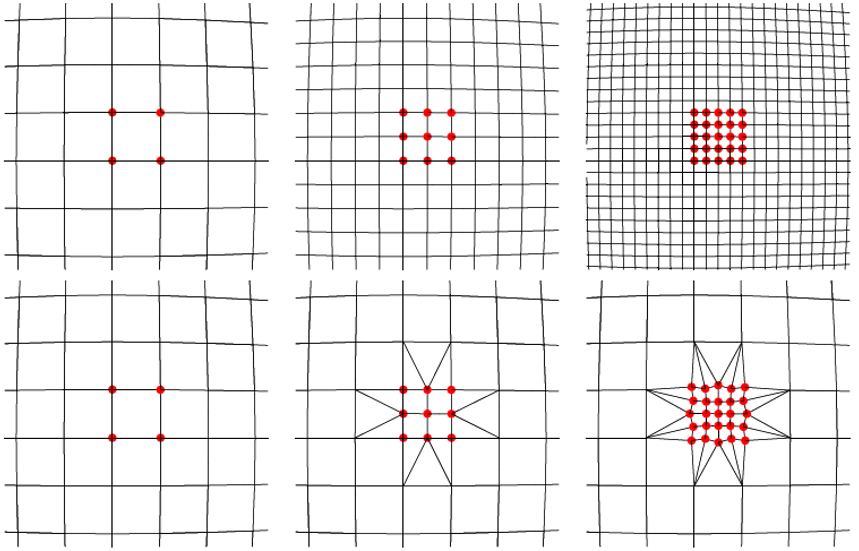
\includegraphics[width=400bp]{q6_pic.png} \\
To make a local subdivision via Catmull-Clark, a simple method is to perform Catmull-Clark, as normal in the local area, but then modify the immediately surrounding barrier to fill-in the gaps of the new edge-vertexes (gaps exist if it is not perfectly flat). \\
To do this, we have to add two edges, (instead of 1 for loop), connecting the new mid-edge point, to the two closest vertices outside the subdivided area. \\
(Note: This is only true for the first subdivision, after this they're triangles, and use the same T-junctions from loop for smoothing to the un-divided area)\\

\item Describe the disadvantages of this simple adaptive subdivision. \\
It creates a lot of 'long' triangles, getting worse as it repeatedly subdivides. \\
It also ends up creating a high difference-of-detail on some vertices. Ex: on the far-right of the picture, the surrounding vertices, some edges go to vertices with valence 4, while some goto vertices with valence 7. This also implies that these are no longer regular, possibly creating extra-ordinary vertices. \\

%This will also make these shapes extra-oridnary for global subdivisions?
\end{enumerate}

\newpage
\end{enumerate}

\end{document}
